%Chapter 3

\chapter{Expost implementation with  interdependent values}  % Main chapter title

\label{Chapter3} % For referencing the chapter elsewhere, use \ref{Chapter2} 

%----------------------------------------------------------------------------------------

% Define some commands to keep the formatting separated from the content 
%\newcommand{\keyword}[1]{\textbf{#1}}
%\newcommand{\tabhead}[1]{\textbf{#1}}
%\newcommand{\code}[1]{\texttt{#1}}
%\newcommand{\file}[1]{\texttt{\bfseries#1}}
%\newcommand{\option}[1]{\texttt{\itshape#1}}


\section{Introduction}
 We try to characterize truthful implementation in ex post equilibrium in this Chapter.  Ex post equilibrium 
 is a good equilibrium in implementation theory for its distribution free property. A large body of literature has been devoted to 
 many aspects of ex post implementation. 

 

 As is pointed out in \parencite{Postlewaite2014}, it is often the case that truthful revelation is not ex post incentive compatible, that is, for a given 
 agent, there are some profiles of the other agents' types for which the agent may be better off by misreporting his type than by 
 truthfully revealing it. However, with the help of money transfer, the authors in \parencite{Maskin00} devised an complicated yet ingenious 
 auction mechanism to Nash implement a class of allocation problems in interdependent value context. It is obvious 
 that money transfer is one key for implementation. 
VCG mechanisms and its extensions are successful mechanisms for dominant strategy implementation in private value context. For interdependent value framework, however
 Here, for a certain but not rare kind of setting, we propose a simple Generalized Vickery mechanism which can easily make the buyers
 reveal their private information truthfully through the help of money transfer. Of course, the Generalized Vickery mechanism is not 
 balanced scheme. Nevertheless, the ability of the mechanism to make people tell truthfully about their private information is a sign of 
 its power.   

  We would like to show the subtlety of those ingenious mechanisms in 
 implementing social goal within our paper's model framework, and how their implemented social goals have satisfied the sufficient and 
 necessary condition.

  
 
 In private value settings, ex post equilibrium is equivalent to dominant strategy
 equilibrium. Thus the well-known VCG mechanism is the ideal mechanism for ex post implementation in private value case. What we care
 most in this chapter is the interdependent value setting. We also assume quasilinear utility for the agents, which is a common 
 assumption. 
 In \parencite{BergemannM08}, the authors focus on identifying conditions for full implementation
 of a social choice set in ex post equilibrium. They stressed that a conceptual advantage of ex post equilibrium is its 
 robustness to the informational assumptions about the environment. \parencite{Maskin00} proposed an indirect bidding mechanism which
 give ex post partial implementation of the socially efficient outcome.
   Another important contribution of \parencite{Maskin00} is that a mechanism for allocating  multiple heterogeneous goods is 
 provided. \parencite{Perry2002} devised another clever mechanism for this case. Their methods consists of a collection of second-price 
 auctions between each pair of bidders conducted over at most two rounds of bidding. Unlike them, in this paper we do not consider 
 full implementation, and for partial implementation we focus on direct revelation mechanism. we use the direct mechanism and manage 
 to cover some more situations that are not implementable using the indirect bidding mechanism in \parencite{Maskin00}.
 We restrict out attention to the conditions garanteeing that truthful revelation of one's own private signal constitutes an ex post 
 equilibrium in some carefully designed direct revelation mechanism. That is, we focus on incentive compatibility of truthful
 information revelation in direct mechanism. Partial implementation is emploed in this paper and henceforth just called implementation.
 In such direct mechanisms,
 a well devised payment rule is of key importance. \parencite{Ausubel99} provides a payment scheme in its generalized Vickery Auction
 mechanism, which under some conditions achieves the task of implementing social efficiency in ex post equilibrium. 
 \parencite{Jehiel2001} considered efficient, Bayes-Nash incentive compatible mechanisms in a social choice setting that allows for informational and allocative externalities(i.e. interdependence exists). They then apply the results to the study of multi-object auctions. We also consider a multi-goods case, but different from their settings in that, each buyer wants one good at most, which are better known as assignment problem in matching theory literature\parencite{Roth1990}. We are also quite different from the matching literature in that we are considering implementation with interdependent values for this problem.

 \parencite{Ely2006} is a work about ex post implementation. However, we provide different formulations which is easier to grasp and applied to different problems.
 
 we first investigate the continuous
 cases of interdependent value,  including allocation of continuous resources and efficient provision of continuous public goods. 
 For example, in a room of dancers, a volume must be chosen for the music so that it can provide the best social efficiency. Each person
 has a valuation function of the form 
 $$u_i= v_i(volume) + \alpha_i\sum_{j\neq i}v_j(volume)$$
 Here, the $\alpha_i$ is the altruist coefficient of agent $i$ , which are known by social planner, only each $v_i()$ is private information. This is a typical interdependent value situation.

 
 %We will see how to implement social efficiency in  later in the paper. 
 


 
 %Our intuition is mainly taken from \parencite{Maskin00} Vickery Mechanism and auction theory. 
Simpleness often means less mistakes. Also, a simple mechanism is  easy to supervise. For an outsider, it is not easy to judge who should win the goods in a very complicated mechanism
, so a corrupted social planner might manipulate the result. That is one motivation for us to construct a direct revelation mechanism.

% In interdependent value settings, a winner often suffers from winners' curse.
%In the following, we first introduce the notion and model
%of interdependent value goods, then for some kind of setting, we find a unique expost Implementation of 
%the socially efficient results. Finally, we find an application of the model in the mineral rights assignment problem by aggregating
%signals in the designed market.




\section{Key concepts and notations}
First, we give some description of the notations used in this chapter. It's similar to the general framework described in the first chapter. In the meantime of depicting the notations here, we give out the settings for this 
chapter in more detail.
The economic environment consists of
$A$: the set of choice possibilities.

$Z=Z_1\times \dots\times Z_n$:the outcome space. For this chapter, implementation with money transfer means that the 
outcome $z$ has the form $(a, t_1,\cdots,t_n)$ where $a$ is from the set of choice possibilities $A$, $t_i$ is 
the payment agent $i$ has to make.

$U=U_1\times \cdots\times U_n$: the set of all admissible utility functions  $u = \{u_i(\cdot, \cdot)\}_{i=1}^n$ whose 
domain is $Z\times S$. In this paper, quasilinearity is assumed, that is , $u_i((a,t), s)$ takes the form $v_i(a,s)-t_i$. 
$v=\{v_i(\cdot, \cdot)\}_{i=1}^n$ is in a space $V=R^+\times R^+$.

$S=S_1\times \cdots\times S_n$: the set of all admissible signals $s=(s_1,\cdots,s_n)\in S$ that determine types of 
parametric utility functions $u_i(\cdot, s)$, and so it is called the space of signals or called the state of the world. 
In many papers, notation $\theta$ is used in stead of $s$. We adopt the notation $s$ of \parencite{Maskin00} in this paper.
Here, apparently both independent value and interdependent value models are both incorporated in this framework.

$E$: a set of  environments(states of the economy) $e=(\{u_i(\cdot, \cdot)\}_{i=1}^n,s)$. In this paper, 
$e=(\{v_i(\cdot, \cdot)\}_{i=1}^n,s)$ since $v_i$ can identify $u_i$. Moreover,
as will be discussed in the information structure part, the $v$ can be elicit out easily by the social
planner, we simply let $e=s=(s_1,\cdots,s_n)$, which is the decentralized information part of the model that need 
mechanism design to tackle.

The information structure of the paper is specified by

(1)$s_i$is privately observed by agent $i$.

(2)$v=\{v_i(\cdot, \cdot)\}_{i=1}^n$ is common knowledge among the agents.To elicit the common
knowledge part of their information, the social planner can adopt methods similar to those \parencite{Repullo90} propose for Nash
implementation of social choice rules. If very agent reports the same, then the result is believed to be the truth. Otherwise,
some kind of punishment is given to everyone.  

Given economic environments, each agent participates economic activities, makes deci-
sions, receives benefits and pays costs on economic activities.The designer wants to reach
some desired goal that is considered to be socially optimal by some criterion. Let

$F:E\rightarrow Z$: the social goal or called social choice correspondence in which
$F(e)$ is the set of socially desired outcomes at a certain state of the economy under some
criterion of social optimality. For this paper, the social goal is denoted
$$F(s)=\{(a^*,t_1,\cdots,t_n)|a^*\ is\ a \ solution\ to \ \max_a \sum_{i=1}^n v_i(a,s)\}$$
We call this the social goal of efficiency in the paper. Since money transfer is not the concerned part.  we can use 
transfers freely to implement the goal.




 

A mechanism consists of a message space and an outcome function. 

$M_i$: the message space of agent i. 

$M=M_1\times \cdots\times M_n$: the message space in which communications take place.

$m_i \in M_i$: a message reported by agent $i$.

$m=(m_1, \cdots,m_n)\in M$: a profile of Messages.

$h:M\rightarrow Z$: outcome functions that translate messages into an outcome.

$\Gamma=\langle M, h\rangle$: a mechanism.

A very important class of mechanisms is the direct revelation mechanism in which $M_i$ is just the possible world state information 
that agent $i$ has. In this paper, the direct revelation mechanism has a message space $M_i=\{(v, s_i)|v\in V, s \in S \}$. The most
important case of $m$ is where all reported $v$ is the same, and for this case the outcome function can be written as 
$h(m)=(a(v,s),t(v,s))$.

Let $b(e, \Gamma)$ be the set of equilibrium messaging strategies that describes the self-interested behavior of individuals.
For instance, Nash equilibrium $N(e,\Gamma)$ is the most frequently adopted equilibrium concept.

A Mechanism $\langle M, h\rangle$ is said to implement a social choice correspondence $F$ in equilibrium strategy 
$b(e, \Gamma)$ on Environment space $E$ if for every $e\in E$, $h(b(e,\Gamma))\in F(e)$.
Incentive compatibility is another way of saying implementation. A Mechanism is said to be incentive-compatible with a social choice
correspondence $F$ on $E$ if it implements $F$ in some kind of equilibrium on $E$. 

\subsection{Ex post equilibrium}

An ex post equilibrium is a Nash equilibrium when every information and strategy choices have been revealed. In an ex post equilibrium, no body will regret the strategy choice he or she has made. In contrast to this, ex ante equilibrium is a Nash equilibrium when not many information has been known by the players. Later on, after everything is known, the participants in an ex ante equilibrium may regret his strategy choice because ex ante equilibrium may not be ex post equilibrium. In this sense, an ex post equilibrium is more robust than an ex ante equilibrium.

We focus on ex post equilibrium $b(\cdot)$ for implementation. According to revelation principle for ex post implementation, if a Mechanism $\langle M, h\rangle$ implements the social choice rule $F$ in ex post equilibrium, then there is a direct revelation mechanism which implements $F$ truthfully in ex post equilibrium(truth telling is an ex post equilibrium) \footnote{This is similar to the revelation principle for dominant strategy implementation. For proofs, see Appendix \ref{Appendix_A}}. This principle narrowes the search space for an ex post implementation mechanism to the space of direct revelation mechanisms, which are the mechanisms we consider in this chapter and the next chapter.

In the analysis of existing mechanisms, the ex post implementable outcomes are sometimes called achievable with perfect manipulation in this paper, because no participant will regret his or her strategical choice in such ex post equilibrium strategy profiles from ex post point of view. The outcomes achievable with perfect manipulation for some CCA(Chinese college admission) mechanisms are discussed in the next chapter on matching. For this chapter, we focus on devising new direct mechanisms to truthfully implement socially efficient choices.







\section{General conditions for implementation with money transfer}



Obviously, for a direct revelation mechanism to implement the social efficiency, every agent must tell truth. 


%We assume outside choice is $a_0$, and $v_i(a_0,s)=v_i(a_0,s_{-i})$, that is, the agent $i$'s value of the outside choice does not
%depend on $s_i$.
\begin{thm} \label{necessary-sufficient}
The social goal of maximizing $\Sigma v_i(a, s)$ can be partially implemented in ex post equilibrium with money transfer if and only if there is a transfer scheme $t(s)$(taken as a tax from agent to the social planner), such that for 
the chosen $a(s)$ maximizing $\Sigma v_i(a, s)$ the following formula holds for all $i$ , $s$ and $s'_i$

\[v_i(a(s), s) - t(s) \geq v_i(a(s'_i, s_{-i}), s) - t(s'_i, s_{-i}) \]
\end{thm}
\begin{proof}
Just use the $t(s)$ as a taxation and according to the definition of ex post equilibrium,  tell truth about one's private signal is an ex post equilibrium.

\end{proof}
The following single crossing condition is a necessary condition of ex post implementation.
It is roughly saying that the value sum of your current type pretending another type(who have different value when truth telling)
and that type pretending your current type is less than the value sum of 
you truthfully report your current type and that other type.

\begin{prop}[single crossing condition]\label{prop}
A social goal of efficiency $G$ can be ex post implememted on $E$  by some mechanism only if $\forall s, \forall v, \forall i$, when 
$v_i(a(v,s), s)\neq v_i(a(v,s'),s')$ where  $s=(s_i, s_{-i})$ and 
$s'=(s'_i, s_{-i})$ (i.e., they only differ in agent's private signal), then

\begin{equation*}\label{equ}
v_i(a(s'),s)-v_i(a(s), s)<v_i(a(s'),s')-v_i(a(s), s')
\end{equation*}

\end{prop}

\begin{proof}
By the necessary and sufficient condition \ref{thm}, there must be a $t(\cdot)$ such that

\[v_i(a(s), s) - t(s) \geq v_i(a(s'), s) - t(s') \]

and

\[v_i(a(s'), s') - t(s') \geq v_i(a(s), s') - t(s) \]

Add the above two inequality together and exchange some terms from both sides, then you get the single crossing condition.


\end{proof}


\section{Continuous social goals}

\subsection{Ex post implementation via VCG}

For two special forms of interdependent value problems, the VCG(Vickery-Clark-Groves) mechanisms can be used to elicit players' truthful reporting of private signal or value in ex post equilibrium. In \parencite{Vickery61},Vickery first proposed the famous second-price sealed bid auction mechanism, which is also called Vickery auction due to his contribution. Later in \parencite{Clark71}, \parencite{Groves73}, taxation scheme in other public choice problems are proposed. The taxation scheme shares similar structures and are later known as VCG mechanisms. However, the VCG mechanism is recognized as a way of eliciting truthtelling in dominant strategy under independent value environment. In the auction theory monograph \parencite{Kris10}, an detailed description of VCG can be found.  In this part, we consider a case that VCG mechanism or adapted VCG mechanism can be used to truthfully implement efficient public choice in ex post equilibrium.

\subsubsection{Value interdependency is through social goal}

Let us discuss with some examples
\begin{example}
 Consider there are two chess players living $L$ miles apart from each other along a road in a city. They drive their cars to meet
 each other every sunday to play chess face to face, and then go back home. Suppose that they can choose anywhere on the road to meet. Let
 $c_i(\cdot)$ be the gasoline cost function for $i$'s one time travelled distance. 
The city governer tries to assign a meeting place minimizing the pollution of their car causing to the city, so he wants to
chose a meeting spot to minimize $c_i(l_i)+c_j(l_j)$. The two chess players all care about the 
pollution but they also care about their oil expenditure, player $i$ feels the disutility $d_i= c_i(l_i)+ \phi_i(c_i(l_i)+c_j(l_j))$, where $\phi_i(\cdot)$ is the polution effect function for $i$, which is monotonically increasing. What
 is the transfer scheme that can make the two players telling truth about their private $c_i$ an ex post equilibrium.
\end{example}
Though it is artificially made, it is indeed interesting to see that there is a tax scheme to accomplish truthful revelation in ex post equilibrium.
That taxation method is to tax agent $t_i= \hat{c}_j(l_j^*)$ and tax agent $t_j=\hat{c}_i(l_i^*)$, where $\hat{c_i(\cdot)},\hat{c_j(cdot)}$ are the reported gasoline cost functions and $l_i^*,l_j^*$ is the social choice, which is a solution to $\min\sum \hat{c}_i(l_i)+\hat{c}_j(l_j)$.

 The total disutility for $i$ is $ t_i+ d_i = c_i(l_i)+\hat{c_j}(l_j)+\phi_i(c_i(l_i)+c_j(l_j))$. If the other player $j$ has told truth about $c_j(\cdot)$, then $ t_i+ d_i = c_i(l_i)+c_j(l_j)+\phi_i(c_i(l_i)+c_j(l_j))$.  Player $i$ wants the total disutility as small as possible, and therefore hopes to get a pair of $l_i,l_j$ to minimize $c_i(l_i)+c_j(l_j)$. However, we know that the social planner chooses $l_i^*,l_j^*$ to minimize $\hat{c_i}(l_i)+\hat{c_j}(l_j)$. Given the other player reported truthfully, i.e.,  $\hat{c}_j=c_j$, player $i$ can let the social planner choose $l_i,l_j$ to minimize $c_i(l_i)+c_j(l_j)$ by just telling truth (let $\hat{c}_i=c_i$).

when extending the two player game of chess to four player game like mahjong, let the four people report their gasoline cost function, the governor choose their play site,
it is also easy to let them tell truth in ex post equilibrium with a well designed taxation. As you can verify, one possible taxation scheme is
$$t_i= \sum_{j\not=i}\hat{c}_j(l_j^*)- \min_{l_j,j\not =i}\sum_{j\not=i}\hat{c}_j(l_j)$$
where $(l_1^*,l_2^*,l_3^*,l_4^*) \text{ is a solution to } \min_{l_k,k\in \{1,2,3,4\}}\sum_{k\in \{1,2,3,4\}}c_k(l_k)$.

\begin{example}
 $n$($n \geq 3$) vegetable firms at $n$ corners of a regular n polygon area transporting their produced goods to a city for sale.
The city planner tries to build the city in a place such that it can minimize the pollution caused by transportation of the goods, 
and the firms cares about its own transportation cost as well as the total pollution\footnote{the reason why a firm care about pollution
may be that the goods are vegetables and pollution can hurt the production}. The oil consumption and thus pollution caused 
by a given amount of goods transportation for each firm is a private value . Each day the goods will be transported to the city once.
What is the taxation scheme that can make each firm report their true private information so that the city 
planner can choose the best place to build the city in order to reduce transporation pollution. Here the meaning of the taxation is not
to reduce pollution directly, but to lead the firms to tell truth about their private information such that the planner can choose a
pollution minimizing choice for building the city.
\end{example}

This is a more realistic economic problem than the previous chess and mahjong problems, and the taxation scheme to let the vegetable firms to report
the true $c_i()$ is
$$ t_i = \sum_{j\not=i}\hat{c}_j(l_j^*)- \min_{l_j,j\not =i}\sum_{j\not=i}\hat{c}_j(l_j) $$

where $(l_1^*,\cdots,l_n^*) \text{ is a solution to }\min_{l_k,k\in \{1,...,n\}}\sum_{k\in \{1,...,n\}}c_k(l_k)$

%The proof of this taxation scheme being able to elicit truthful reports is similar to the reasoning in the above example.
%and is relegated to the Appendix \ref{Appendix_C}.




\begin{remark}
A feature of VCG taxation scheme is retained in the above problems. The scheme taxes player $i$ the aggravation of gasoline consumption that the participation of him or her causes to the other players.
  
\end{remark}


\subsubsection{Value interdependency is through a known altruistic inclination}

In the beginning of this chapter, we have given a dancers example. Let us revisit it. In a room of dancers, a volume must be chosen for the music so that it can provide the best social efficiency. Each person
 has a valuation function of the form 
 $$u_i= v_i(volume) + \alpha\sum_{j\neq i}v_j(volume)$$
 Here, the $\alpha$ is the altruist coefficient of all the agents , which is known by the social planner, only each $v_i()$ is private information. This problem is an interdependent value problem. Suppose the social planner aims to choose a music volume to maximize $\sum_{i\in \{1,\cdots,n\}} u_i(volume)$.

 An adapted VCG mechanism can be devised to elicit every dancer's true report of $v_i()$. After receiving the reports $\hat{v_1},\cdots,\hat{v_n}$, the social planner find a solution $volume^*$ to $\max_{volume}\sum_{i\in \{1,\cdots,n\}}\hat{v}_i(volume)$ because $\sum_{i\in \{1,\cdots,n\}} \hat{u}_i(volume)=(1+(n-1)\alpha)\sum_{i\in \{1,\cdots,n\}} \hat{v}_i(volume)$. The taxation is
 $$t_i=(1-\alpha)(\max_{volume}\sum_{j\not=i}\hat{v}_j(volume)-\sum_{j\not=i}\hat{v}_j(volume^*))$$

 The total welfare for $i$ is $ u_i-t_i= v_i(volume^*) + \alpha\sum_{j\neq i}v_j(volume^*)+ (1-\alpha)\sum_{j\not=i}\hat{v}_j(volume^*)- (1-\alpha)\max_{volume}\sum_{j\not=i}\hat{v}_j(volume)$. If the other player $j$ has told truth about $v_j(\cdot)$, then $  u_i-t_i = \sum_{i\in \{1,\cdots,n\}} v_i(volume^*)-(1-\alpha)\max_{volume}\sum_{j\not=i}v_j(volume)$, the term after $-$ is independent with $\hat{v}_i$.   However, we know that the social planner chooses $volume^*$ to maximize $\sum_{i\in \{1,\cdots,n\}}\hat{v}_i(volume)$. Given the other player reported truthfully, i.e.,  $\hat{v}_j=v_j, j \not = i$, player $i$ can let the social planner choose $volume^*$ to maximize $\sum_{i\in \{1,\cdots,n\}} v_i(volume)$ by just telling truth (let $\hat{v}_i=v_i$).

 \begin{remark}
   Truthful implementation in ex post equilibrium under this kind of interdependent altruistic utility function is very demanding. It needs the altruist parameter $alpha$ being the same across the agents. Only with this requirement fulfilled, can the problem be implemented by the above adapted VCG mechanism.This same $alpha$ can be interpreted as a general altrustic inclination among a group of similar people. 
 \end{remark}

 
 \subsection{Uniqueness of transfer scheme for continuously differentiable cases}

First, an economical problem is provided. 
\begin{example}
A country has N oligopoly firms producing the same goods ,say oil. They face an exogenous demand function. Competition among them hurt
aggregate profits of the firms. 
The country want to devise a taxation scheme such that every firm reveal their true production cost so that the country can plan
the production quantity for each firms to maximize total profit of the country. This is the private value case that can be implemented
using classical VCG mechanism. 

Now change the scenario to another case where the firms' CEOs know the private cost informations of their own firms. They are all 
shareholders, and all have a large percent of their own firm's stock and a different amount of share on other firms, and these shares
are common knowledge.  Now the valuation of each firm's CEO on the country's production assignment plan are dependent upon all
the cost information and each firm's final production quantity as specified by the country.
\end{example}
 
The taxation scheme is a new challenge. We try to face this kind of challenge by designing mechanisms to implement a social goal in ex post equilibrium with money transfer(suitable taxation). For those that can be implemented with money transfer, we give the taxation scheme that can be used to implement the socially efficient choice.

One interesting finding is that the money transfer scheme is unique up to a shifting constant if the functions involved are
continuously differentiable as to the private signal.

\begin{lemma}
  \label{l1}
Assuming all the partial derivatives exists and are continuous, then solve the following 
differential equations
 $$\frac{\partial t_i}{\partial s_i} = \frac{\partial v_i(a(s_i,s_{-i}),s_i,s_{-i})}{\partial a } \frac{\partial a}{\partial s_i}$$
 $i=1,\cdots,n$ 
 
 gives us a transfer scheme $t(\cdot)$.
A sufficient and necessary condition for implementation with money transfer in such continuous case is that, for all $i$,$s$
by shifting up or down the $t(\cdot,s_{-i})$ to let it be tangent with $ v_i(a(\cdot,s_{-i}),s_i,s_{-i})$ at $s_i$, the curve
$t_i(\cdot,s_{-i})$ is below $ v_i(a(\cdot,s_{-i}),s_i,s_{-i})$, namely, $v_i(a(\cdot,s_{-i}),s_i,s_{-i})-t(\cdot,s_{-i})$ is
maximized at $s_i$. 
\end{lemma}
\begin{proof}
 If truth telling is a ex post equilbrium, it must be the case that $s_i$ is the solution to
 $$\max_{s'_i} \{v_i(a(s'_i,s_{-i}),s_i,s_{-i})-t(s'_i,s_{-i})\}$$
 solving it, we get the conclusions in the theorem.
\end{proof}

Thus for any two $t_i,t_i'$ which can lead to truthful implementation in ex post equilibrium, $\frac{\partial(t_i-t_i')}{\partial s_i}=0$, and we have the uniqueness of transfer.

From Lemma \ref{l1}, the uniqueness theorem followes.
  \begin{thm}(Uniqueness)
    If a mechanism with money transfer exists which truthfully implements the social efficiency in  ex post equilibrium, then given any $s_{-i}$,  the transfer tax scheme $tax(x)=t_i^*(x,s_{-i})$ for agent $i$ is essentially the tangent curve of $i$'s profit function family  $f(x,s_i)=v_i(a(x,s_{-i}),s_i,s_{-i}) $ where $s_i, x \in S_i$, that is, $tax(x)$ has the same slope as $f(x,s_i)$ at $s_i$. Moreover, any other implementing scheme is an upward or downward shift of it, ie., $tax(x)=t_i^*(x,s_{-i}) + c(s_{-i})$.
  \end{thm}

The theorem is simple, but it contains much information. One thing is that not every continuously differentiable
social goal $a(s)$ is implementable in ex post equilibrium with money transfer. It must satisfy the conditions in the theorem 
to be implemented with money transfer, that is, there must be an upper envelope curve for a family of function curves. The second thing is that even if it can be implemented with money transfer, the scheme for 
implementing it is unique in essence. They only differ by a constant\footnote{the solution to the differential equations are some specific
  function plus something of the form $c(s_{-i})$ that is not changing with $s_i$}. The model here does not include
the previous VCG mechanism case as $c_i$ or $v_i$ are functions there, not a $s_i$. The idea to convey is that $i$'s transfer difference of any two mechanisms truthfully implementing an efficient social goal must be a function which is not changing with the reported value of $i$. 

Now let us consider the oil producers example again. We should give a mathematical structure to it in order to show how the process of mechanism
design is done in this case. Market demand function is $q(p)$, inverse demand function is $p(q)$. The cost function 
facing firm i is $c(q_i,s_i)$, the parameter $s_i$ is privately known. The share of firm $j$
that the leader of firm  $i$ holds is $m_{ij}$, and  the leader $i$ cares the overall profit 
$v_i(q,s)=\sum_{j=1}^{n} m_{ij}(q_jp(q)-c(q_j,s_j))$. The country's goal is 
$$\max_{\{q_1,\cdots,q_n\}}\sum_{j=1}^{n} (q_jp(q)-c(q_j,s_j)) $$
The solution to this maximization problem must satisfy the first order conditions
$$q_j \frac {\partial p(q)}{\partial q}+p(q)=\frac {\partial c(q_j,s_j)}{\partial q_j}$$
$$j=1,\cdots,n$$

For many function forms, the above conditions are also sufficient, and we calculate out ${q_1(s),\cdots,q_n(s)}$ from the above 
equations. Next, by using the conditions in the above theorem, we get 
$$\frac{\partial t}{\partial s_i} = \sum_{j=1}^{n} m_{ij}\{q_j\frac {\partial p(q)}{q}(\frac{\partial q_1}{s_i}+\cdots+\frac{\partial q_n}{s_i})-\frac {\partial c(q_j,s_j)}{\partial q_j}\frac{\partial q_j}{s_i}\}$$
Now that the transfer scheme is calculated, we only need to verify whether it satisfies the requirement that for all $i$,$s$,  $s_i$ maximizes  
$$\sum_{j=1}^{n} m_{ij}\{q_j(\cdot,s_{-i})p(q(\cdot,s_{-i}))-c(q_j(\cdot,s_{-i}),s_j)\}-t_i(\cdot,s_{-i})$$
When the requirement holds, then $t$ is the money transfer scheme.

To have an intuitionistic idea about the above discussion, we will give a numerical illustration. Let $n=2,p(q)=5-q, m_{11}=2/3,m_{12}=1/3$, $c(q,s_i)=qs_i$ for $i=1,2$. Suppose that the agent 2 has reported the real $s_2=1$. Now what is $tax(x)$ for agent 1 which can make him or her tell truth?

A possible tax scheme for player 1 is $tax(x)=x^2/9 - 2x/9 + 1$, which can be deduced from the just sketched method.\footnote{We use the software Maxima to calculate the functions and draw the graph. A detailed guide for doing such jobs is obtained from \parencite{Maxima}.
  See the Appendix \ref{Appendix_B} for the code of producing the graph.}

In the graph, we depict the tax curve $tax(x)$ together with the family of $f(x,s_1)$s that is parallel to it\footnote{Tangent after an appropriate downward shift.} at five $x$s  $(0.1,1.0,1.2,1.8,3)$. If $S_i= (0,3]$, then the $tax(x)=x^2/9 - 2x/9 + 1$ is individual rational for the agent 1. We can also see that only $tax(x)$ is convex while all the family of $f(x,s_1)$s with $s_1$ changing from $0$ to $3$ are concave. Therefore it is a tax scheme which can make the agent 1 tell truth as shifting any curve $f(x,s_1)$ downward such that it is tangent to $tax(x)$ at $s_1$ will make the curve  $f(x,s_1)$ lie under $tax(x)$. As for the agent 2, the taxation is similarly calculated given any $s_1, m_{21},m_{22}$ and we omit it here.



%\begin{figure}[htb]
%     \centering
%     \includegraphics[scale=0.5,bb=0 0 385 567]{picture.png}
%     \caption{Some description about the picture}
%     \label{picture-label}
%     \end{figure}

 \begin{figure}
\centering
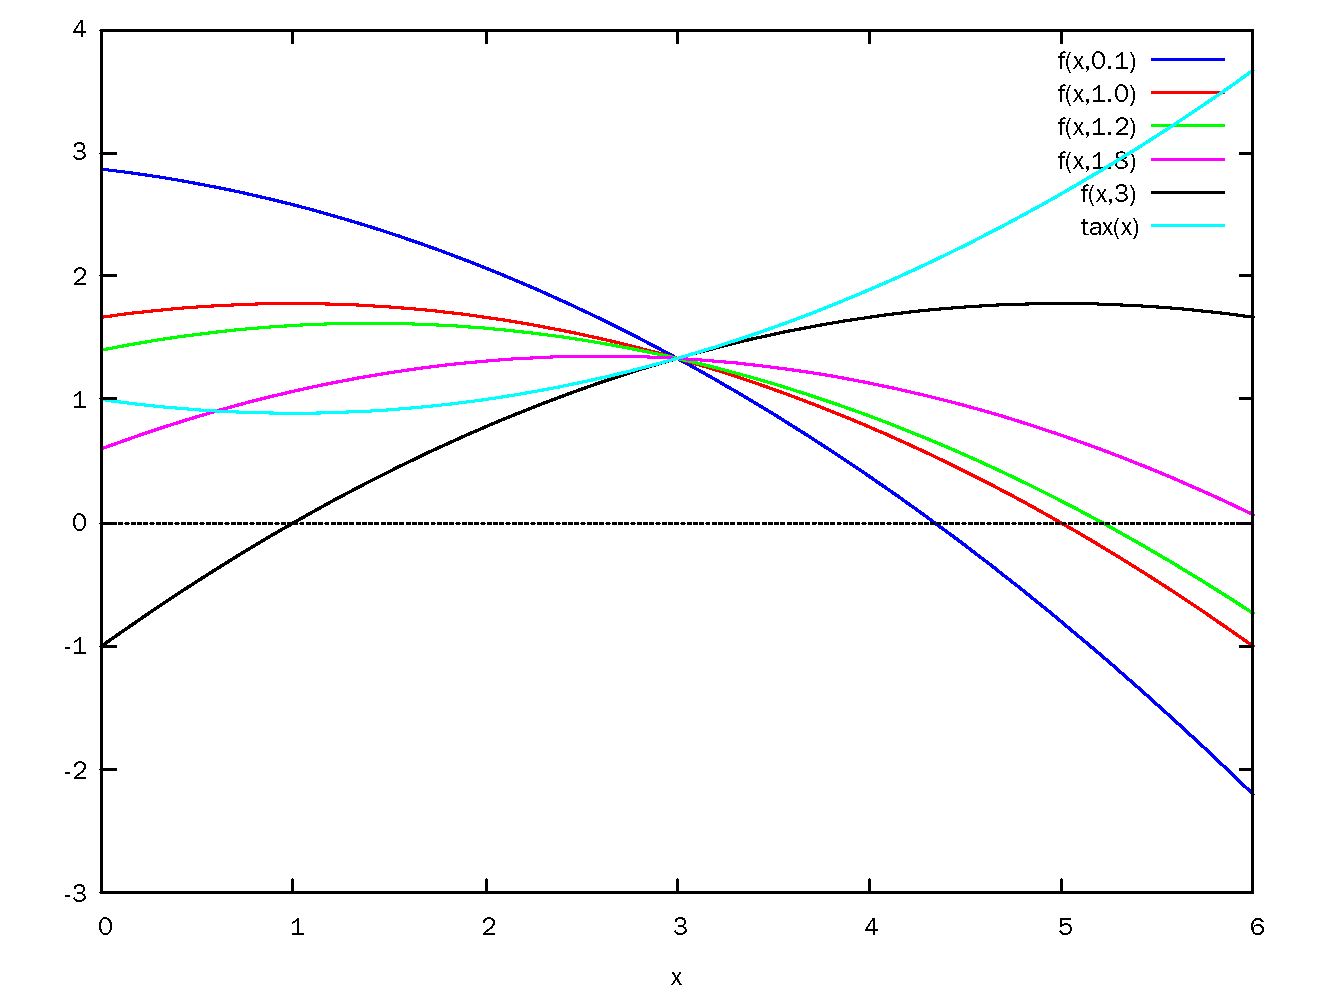
\includegraphics[width = 11cm]{tax.pdf}
\caption{tax scheme $tax(x)$ etc.} \label{fig:tax}
\end{figure}

For this continuously differentiable situation, the private value case of the problem always has the unique solution, the uniqueness
has been shown by the above more general result. And the unique mechanism is the well-known VCG mechanism. This has been shown by
Laffont and Maskin(Econometrica, 1980). 

%And for private value case, 
%ex post implementation is indeed dominant strategy implementation. A specialness of the private value situation is that the calculated
%VCG money transfer mechanism can always satisfy the additional requirement for implementability. We will show why now. 
\section{Discrete social goal}
The discrete social choice possibility set $A$ does not allow differential analysis like we do above in the continuous social choice
possibility set case. However, the allocation of discrete social resources, or the determination of whether a project should be carried
are important social choice problem we have to face. We are also interested at whether we can implement such social choices with money
transfer. We start from allocation of one good.

\subsection{Allocation of one good  }

Imagine the following scenario : there is a group of agents who are familiar with each other, and the social planner has
one good to allocate to one of them. The socially efficient outcome is to give it to the one who 
values it the most. Suppose each agent can only detects one of the qualities of the good, and the total value of the 
good for any agent is only determined by all the qualities of the good and the importance of each quality to the agent 
himself. This is a situation completely covered by our model framework in the previous section. The social choice possibility
set $A=\{(1,0,\cdots,0),\cdots,(0,\cdots,0,1)\}$. Every body only cares about getting the object, and when one does not get it his or
her utility gain is 0 from the allocation. Now what the social planner want is a mechanism to implement the socially efficient outcome. 

\parencite{Maskin00} has partly solved the problem and give us an auction mechanism to implement a rather large economic 
environment set $E$ in this one good allocation environment. However, as the authors pointed out in the footnote 26 of 
their paper, some utility forms can not be implemented by their auction mechanism. In this section, through combining the 
insights of the two authors with the power of revelation mechanism, we try and find a direct revelation mechanism  which
enlarge the $E$ on which the social goal of efficiency $G$ is implementble, for example, the economic environment in footnote
26 of their paper.
In Theorem~\ref{necessary-sufficient}, we have shown what is the sufficient and necessary condition for implementation with money 
transfer. In this simple case, we give some simple assumptions parallel to the sufficient and necessary condition
so that we can implement the social efficiency.

In this one good allocation problem,let $v_i(s)=v_i(\epsilon_i,s)$ where $\epsilon_i$ is the allocation of the good to i. Then we
have the following sufficient condition for ex post implementation of efficient result in an auction.
\begin{prop}
The efficient allocation of one good can be implemented  as an ex post equilibrium
if  
 $$\forall i,\forall s_{-i}, \exists s_i^* \in S_i, such\ that $$
 $$(a) v_i(s_i^*, s_{-i}) = max_{j\not = i} v_j(s_i^*, s_{-i}); $$
 $$(b) When\ v_i(s_i, s_{-i}) > v_i(s_i^*, s_{-i}), $$
  $$\forall j \not = i, v_i(s_i, s_{-i}) - v_i(s_i^*, s_{-i}) > v_j(s_i, s_{-i}) - v_j(s_i^*, s_{-i});$$
  $$When\ v_i(s_i, s_{-i}) < v_i(s_i^*, s_{-i}), $$
  $$\forall j \not = i, v_i(s_i, s_{-i}) - v_i(s_i^*, s_{-i}) < v_j(s_i, s_{-i}) - v_j(s_i^*, s_{-i});  $$
 
\end{prop}
\begin{proof}
The proof is through  constructing the needed mechanism and then examining how the mechanism works in all possible situations.
We only need to find an appropriate mechanism to implement it. Now we give it as follows and then prove it can indeed
 implement the social goal of efficiency.
 
 Step 1. Every agent reports a $(v,s_i)$ from the set $V\times S_i$;
 
 Step 2. If the $v$ reported by every agent has some disagreement, then the result is that no body gets the good.
 
 Step 3. If the $v$ reported by every agent is the same, then solve the maximization problem 
 $$\max_{i \in \{1,\cdots,n\}}v_i(s)$$
 and give the good to the solution agent. The winner pays $v_i(s_i^*, s_{-i})$ 
 which $s_i^*$ is the solution to the following minimization problem
 \begin{equation}
 \min_{s_i^*\in S_i} v_i(s_i^*, s_{-i})\quad
 s.t.\quad  v_i(s_i^*, s_{-i})\geqslant \max_{j\neq i, j \in \{1,\cdots,n\}} v_j(s_i^*, s_{-i})
 \end{equation}\label{pay}
Explanation of this mechanism being able to induce truthful revelation of every agent's private signal is not
difficult with the help of case analysis for all possibilities.

Devide the actually received signal $s_i^*$ into three cases:

(i)When $v_i(s_i, s_{-i})> v_i(s_i^*, s_{-i})$, given others truthfully revealing their private signals $s_{-i}$, the agent i
wishes to win the auction. Truthful revelation of $i$'s private signal is enough to insure the win, since the $s_i^*$
is enough to guarantee a tied first according to assumption (a), further by the first part of assumption (b), the true $s_i$ gives
agent $i$ the clear first. Therefore truthful revelation of the signal $s_i$ in this case is incentive compatible.

(ii)When $v_i(s_i, s_{-i})< v_i(s_i^*, s_{-i})$, given others truthfully revealing their private signals $s_{-i}$, the agent i's best choice is to lose the auction.
Truthful revelation of $i$'s private signal is sure to make him lose the auction, since  the $s_i^*$ only gives him a tied first according to assumption (a), 
further by the second part of assumption (b), the true $s_i$ will not make him the first. Therefore truthful revelation of the signal $s_i$ in this case is also incentive compatible.

(iii)When $v_i(s_i, s_{-i}) = v_i(s_i^*, s_{-i})$, given others truthfully revealing their private signals $s_{-i}$, winning or losing the auction has the same net value of 0. 
Therefore truthful revelation of the signal $s_i$ in this case is incentive compatible trivially.

\end{proof}




The improvement of our mechanism on \parencite{Maskin00} is that they have four assumptions for implementation, but we only need two 
assumptions which are essentially parallel to their first three assumptions and less demanding. 

Their three assumptions are listed below.

(i)$\frac{\partial v_i}{\partial s_i} > 0$;

(ii) $\forall i, j \not = i, \frac{\partial v_i}{\partial s_i}(s_1,...,s_n)
> \frac{\partial v_j}{\partial s_i}(s_1,...,s_n)$,

at any point where $v_i(s_1,...,s_n) = v_j(s_1,...,s_n)= max_k v_k(s_1,...,s_n)$;

(iii)$ \forall s_{-i} \in S_{-i}, \exists s_i' \in S_i, such\ that\ v_i(s_i', s_{-i}) > max_{j\not=i}v_j(s_i', s_{-i})$.


Therefore, we can implement social
 goal of efficiency on all the economic  environments $E$ that their auction mechanism can implement and can implement beyond their
 scope. As a demonstration of the power of our direct revelation mechanism as shown in the proof, we now implement the efficiency 
 goal for \parencite{Maskin00} footnote 26.
 
\begin{example}[Footnote 26 of the paper Efficient Auctions]
$$v_1(s_1,s_2)=s_1-2s_2+5$$
$$v_2(s_1,s_2)=s_2-\frac{1}{2}s_1+5$$
The $v$ clearly satisfy Assumption 1 and 2, therefore it is implementable using our direct revalation mechanism described above. By
using the minimization value in Formula~\ref{pay}, we get the pay that the winner has to make,  which is a constant $5$. It is easy to verify that truthful report is a Nash Equilibrium.
 
\end{example}
For the above example, the reason why the auction in \parencite{Maskin00} cannot implement social goal of efficiency, is perhaps that 
their contingent biding function loses the information revelation role in this case, since 
$b_1(v_2)=15-2v_2,\quad b_2(v_1)=\frac{15-v_1}{2}$.

The next section will be with multiple goods, and there we will provide a sufficient condition for ex post implementation. When that condition is applied to the one object case($1$ is a special case of $n$), we will have a further relaxed condition than the one we proposed in this part.
\subsection{Assignment of multiple goods}
\label{sec:assignment_of_multiple_goods}

For allocation of multiple goods under interdependent value environment, not much has been done to our knowledge. \parencite{Che2015} involve assigning indivisible objects to individuals without monetary transfer under interdependent values setting. Now in this subsection we extend the previous result to the allocation of multiple goods with money transfer under interdependent value environment.  The problem we'll consider is actually the assignment model with a special kind of interdependency. \footnote{For the private value assignment problem, the knowledge of which may help the understanding of this section, see Chapter 8 \parencite{Roth1990}for reference.} 

Suppose that there are $m$ agents and $n$ goods such that $m > n$. Each agent can get at most one object.   Agent $i$'s valuations of the n goods is given by $(v_{i1}(s),v_{i2}(s),...,v_{in}(s))$ respectively, where $s=(s_1,s_2,...,s_m)$ is a vector of signals held privately by agent $1$,agent $2$,..., agent $m$ respectively. Allocation result is a $m \times n$ matrix $X$ where $\sum_{i\in\{1,...,m\}}x_{ij} \leq 1 \text{ for all } j$ and  $\sum_{j\in\{1,...,n\}}x_{ij} \leq 1 \text{ for all } i$. The social goal is to allocate the goods to maximize the social efficiency $\sum_{ij}x_{ij}v_{ij}(s)$.

This problem is generally not ex post implementable. However, we find under the following condition, we can design a mechanism to implement the socically efficient goal in ex post equilibrium.

Condition $\rho$:

$\forall i,\forall s_{-i}, \exists s_i^*$,for all $k \in \{1,\cdots,n\}$, such that :

from the maximizing solution $x$s to  $\sum_{ij}x_{ij}v_{ij}(s)$, one can designate an allocation scheme, such that

%if $s_i = s_i^*$, agent $i$ will be given the certain good $k$ or have no good allocated in a value maximizing allocation schemes.

if $v_{ik}(s_i) < v_{ik}(s_i^*)$, agent $i$ will have no probability to be allocated the good $k$. %in all the maximizing allocation schemes.

if $v_{ik}(s_i) > v_{ik}(s_i^*)$, agent $i$ will have a probability to be allocated the certain good $k$ and charged $ v_{ik}(s_i^*)$. However, the probability does not depend on $s_i$. % in all the maximizing allocation schemes.


\begin{proof}
  The proof is through  constructing the needed mechanism and then examining how the mechanism works in all possible situations.
  
We first need to find an appropriate mechanism. Now we give it as follows and then prove it can indeed implement the social goal of efficiency.
 
 Step 1. Every agent reports a $(v,s_i)$ from the set $V\times S_i$.\footnote{Here $v$ is the matrix
   \begin{matrix}
     v_{11}& \cdots & v_{1n}\\
     \vdots& \ddots & \vdots\\
     v_{m1}& \cdots & v_{mn}
   \end{matrix}
   , where $v_{ij}$ is the value function of agent $i$ getting good $j$.
 }
 
 Step 2. If the $v$ reported by every agent has some disagreement, then the result is that no body gets any good.
 
 Step 3. If the $v$ reported by every agent is the same, then to allocate the goods, choose the social value maximizing allocation scheme designated in Condition $\rho$ which satisfy the additional two assumptions in it.
 
 
 
 
Explanation of this mechanism being able to induce truthful revelation of every agent's private signal is not
difficult with the help of case analysis for all possibilities.

For any $k$, devide the actually received signal $s_i$ into three cases:

(i)When $v_{ik}(s_i, s_{-i})> v_{ik}(s_i^*, s_{-i})$, given others
truthfully revealing their private signals $s_{-i}$, the agent i
wishes to be assigned good $k$ to gain $v_{ik}(s_i, s_{-i})- v_{ik}(s_i^*, s_{-i})$ surplus. Truthful revelation of $i$'s private signal gives $i$ a probability of the assignment of $k$ to $i$, since $s_i$ will not influence this probability,
truthful revelation of the signal $s_i$ in this case is incentive
compatible.\footnote{Not influencing probability is important, because if not, agent $i$ would have incentive to manipulate the probability by report a false $s_i$.}

(ii)When $v_{ik}(s_i, s_{-i})< v_{ik}(s_i^*, s_{-i})$, given others
truthfully revealing their private signals $s_{-i}$, the agent i wishes not to be allocated the good and being charged
$v_{ik}(s_i, s_{-i})< v_{ik}(s_i^*, s_{-i})$. Truthful
revelation of $i$'s private signal $s_i$ is enough to insure that he
is not allocated good $k$ by Condition $\rho$.  truthful revelation
of the signal $s_i$ in this case is also incentive compatible.

(iii)When $v_{ik}(s_i, s_{-i}) = v_{ik}(s_i^*, s_{-i})$, given others
truthfully revealing their private signals $s_{-i}$, winning or losing
the assignment of good $k$ has the same net value of 0. Therefore
truthful revelation of the signal $s_i$ in this case is incentive
compatible trivially.

Therefore, truthful revelation is incentive compatible overall for this mechanism.

\end{proof}

Condition $\rho$ does not seem to be easy to satisfy. Nevertheless, in
the following we give a more concrete $v$ which satisfy Condition
$\rho$ to show that it is indeed satisfiable in some situations so
that we can ex post implement the socially efficient goal.
\begin{prop}
  \label{rho}
  The social efficient goal of $\max_{x}x_{ij}v_{ij}(s)$ can be ex post implemented if:
For all $i$ and $j$,
$$v_{ij}=b_{ij} + o_i(s_i) + \sum_{l \not = i} r_l(s_l) $$
where $b_{ij}>0$ is the base value, $s_i \in [0, + \infty)$, $\forall i,o_i(0)=r_i(0)=0$

Assumptions are listed below.

(i)For all $i$, $\frac{\partial o_i}{\partial s_i} > 0$, $\frac{\partial r_i}{\partial s_i} > 0$;

(ii) $\forall i, \frac{\partial o_i}{\partial s_i}
> \frac{\partial r_i}{\partial s_i}$;

%(iii)Faced with a $s_{-i}$, as the $s_i$ increases, agent $i$ will finally get some good allocated in the solution of the assignment problem.
\end{prop}


The intuition of these assumptions implying Condition $\rho$ is that
the own effect of a signal $s_i$ is larger than its effect to the rest
of the agents. And therefore there exists a threshold $s_i^*$ as
required by Condition $\rho$ for agent $i$ to get into the group of
good winners. As for the fixedness of the good winning probability by agent $i$,
it's in part due to the fact that as $s_i$ increases, the increasing
rate of $v_{ik}$ is at least as large as any other $v_{ab}$, where
$ab$ stands for arbitrary agent and good combination not equal to
$ik$. The formal proof can be seen in Appendix \ref{Appendix_C}.







\section{Conclusion}

We have focused on designing mechanisms implementing social goals truthfully in ex post equilibrium. The one caveat is that there may be collusions among the players. The way to deter this is to form laws against such behaviors globally or to negotiate on contracts against such behaviour locally. Why not just form laws against lying and save all the efforts of designing incentive compatible mechanisms ? The answer is that lying by a person is much harder to detect than collusion by a groups of people, and we can hardly penalize lying with law due to lackness of concrete evidence.

The whole chapter builds on the assumption of quasilinearity of agents' value function. Under such preference,  money can be utilized 
as a tool to help elicit true information about the world that are scattered among the agents.
When the mechanism designer cares more on efficiency than fairness, our mechanism is ideal. Since the redistributional effect of money 
transfer has no influence on the aggregate social value.

%----------------------------------------------------------------------------------------




%----------------------------------------------------------------------------------------

